\documentclass{beamer}
\usepackage{graphicx} % Required for inserting images
% \usepackage[latin2]{inputenc}
\usepackage{amsmath}
\usepackage{mathtools}
\usepackage[shortlabels]{enumitem} % for {enumerate}[a]
%\usepackage[pdftex]{graphicx}
\usepackage{amsfonts}
\usepackage{amssymb}
%\usepackage{fancyhdr}
\usetheme{Madrid}
%\pagestyle{fancyplain}
\usepackage{mathrsfs}  
\usepackage{setspace}
\usepackage{epsfig}
\usepackage{color}
\usepackage{tikz}
%\usepackage{UVMThesisStyle-July2020}
%\usepackage{cancel}
\usepackage{float}
%\usepackage{cite}
\usepackage{url}


%my own packages
\usepackage{latexsym}
\usepackage{amssymb}
\usepackage{amsthm}
\usepackage{amscd}
\usepackage{amsmath}
\usepackage{tikz-cd}
\usepackage{soul}
\usepackage{subfiles}


%theorem style commands
%\newtheorem{theorem}{Theorem}[section]
%\newtheorem{fact}[theorem]{Fact}
%\newtheorem{claim}[theorem]{Claim}
%\newtheorem{lemma}[theorem]{Lemma}
%\newtheorem{definition}[theorem]{Definition}
%\newtheorem{proposition}[theorem]{Proposition}
%\newtheorem{corollary}[theorem]{Corollary}
%\newtheorem{conjecture}[theorem]{Conjecture}
%\newtheorem{hypothesis}[theorem]{Hypothesis}
%\newtheorem{example}[theorem]{Example}
%\newtheorem{remark}[theorem]{Remark}


%\theoremstyle{remark}
\newtheorem{case}{Case}

\numberwithin{equation}{section}
\numberwithin{case}{theorem}

%shortcuts
\newcommand{\cA}{\mathcal{A}}		%curly a
\newcommand{\cB}{\mathcal{B}}		%curly b
\newcommand{\cC}{\mathcal{C}}		%curly c
\newcommand{\cD}{\mathcal{D}}		%curly d
\newcommand{\cE}{\mathcal{E}}		%curly e
\newcommand{\cF}{\mathcal{F}}		%curly f
\newcommand{\cG}{\mathcal{G}}		%curly g
\newcommand{\cH}{\mathcal{H}}		%curly h
\newcommand{\cI}{\mathcal{I}}		%curly i
\newcommand{\cJ}{\mathcal{J}}		%curly j
\newcommand{\cK}{\mathcal{K}}		%curly k
\newcommand{\cL}{\mathcal{L}}		%curly l
\newcommand{\cM}{\mathcal{M}}		%curly m
\newcommand{\cN}{\mathcal{N}}		%curly n
\newcommand{\cO}{\mathcal{O}}		%curly o
\newcommand{\cP}{\mathcal{P}}		%curly p
\newcommand{\cQ}{\mathcal{Q}}		%curly q
\newcommand{\cR}{\mathcal{R}}		%curly r
\newcommand{\cS}{\mathcal{S}}		%curly s
\newcommand{\cT}{\mathcal{T}}		%curly t
\newcommand{\cU}{\mathcal{U}}		%curly u
\newcommand{\cV}{\mathcal{V}}		%curly v
\newcommand{\cW}{\mathcal{W}}		%curly w
\newcommand{\cX}{\mathcal{X}}		%curly x
\newcommand{\cY}{\mathcal{Y}}		%curly y
\newcommand{\cZ}{\mathcal{Z}}		%curly z

\newcommand{\sA}{\mathscr{A}}		%script a
\newcommand{\sB}{\mathscr{B}}		%script b
\newcommand{\sC}{\mathscr{C}}		%script c
\newcommand{\sD}{\mathscr{D}}		%script d
\newcommand{\sE}{\mathscr{E}}		%script e
\newcommand{\sF}{\mathscr{F}}		%script f
\newcommand{\sG}{\mathscr{G}}		%script g
\newcommand{\sH}{\mathscr{H}}		%script h
\newcommand{\sI}{\mathscr{I}}		%script i
\newcommand{\sJ}{\mathscr{J}}		%script j
\newcommand{\sK}{\mathscr{K}}		%script k
\newcommand{\sL}{\mathscr{L}}		%script l
\newcommand{\sM}{\mathscr{M}}		%script m
\newcommand{\sN}{\mathscr{N}}		%script n
\newcommand{\sO}{\mathscr{O}}		%script o
\newcommand{\sP}{\mathscr{P}}		%script p
\newcommand{\sQ}{\mathscr{Q}}		%script q
\newcommand{\sR}{\mathscr{R}}		%script r
\newcommand{\sS}{\mathscr{S}}		%script s
\newcommand{\sT}{\mathscr{T}}		%script t
\newcommand{\sU}{\mathscr{U}}		%script u
\newcommand{\sV}{\mathscr{V}}		%script v
\newcommand{\sW}{\mathscr{W}}		%script w
\newcommand{\sX}{\mathscr{X}}		%script x
\newcommand{\sY}{\mathscr{Y}}		%script y
\newcommand{\sZ}{\mathscr{Z}}		%script z

\newcommand{\bbA}{\mathbb{A}}		%bold a
\newcommand{\bbB}{\mathbb{B}}		%bold b
\newcommand{\bbC}{\mathbb{C}}		%bold c
\newcommand{\bbD}{\mathbb{D}}		%bold d
\newcommand{\bbE}{\mathbb{E}}		%bold e
\newcommand{\bbF}{\mathbb{F}}		%bold f
\newcommand{\bbG}{\mathbb{G}}		%bold g
\newcommand{\bbH}{\mathbb{H}}		%bold h
\newcommand{\bbI}{\mathbb{I}}		%bold i
\newcommand{\bbJ}{\mathbb{J}}		%bold j
\newcommand{\bbK}{\mathbb{K}}		%bold k
\newcommand{\bbL}{\mathbb{L}}		%bold l
\newcommand{\bbM}{\mathbb{M}}		%bold m
\newcommand{\bbN}{\mathbb{N}}		%bold n
\newcommand{\bbO}{\mathbb{O}}		%bold o
\newcommand{\bbP}{\mathbb{P}}		%bold p
\newcommand{\bbQ}{\mathbb{Q}}		%bold q
\newcommand{\bbR}{\mathbb{R}}		%bold r
\newcommand{\bbS}{\mathbb{S}}		%bold s
\newcommand{\bbT}{\mathbb{T}}		%bold t
\newcommand{\bbU}{\mathbb{U}}		%bold u
\newcommand{\bbV}{\mathbb{V}}		%bold v
\newcommand{\bbW}{\mathbb{W}}		%bold w
\newcommand{\bbX}{\mathbb{X}}		%bold x
\newcommand{\bbY}{\mathbb{Y}}		%bold y
\newcommand{\bbZ}{\mathbb{Z}}		%bold z

\newcommand{\rI}{\mathrm{I}}
\newcommand{\rII}{\mathrm{II}}


\newcommand{\Proj}{\operatorname{Proj}} 	%Proj
\newcommand{\sProj}{\operatorname{sProj}} 	%sProj
\newcommand{\res}{\mathrm{res}} 	%res
\newcommand{\Hom}{\operatorname{Hom}} 	%Hom
\newcommand{\GL}{\mathrm{GL}} 	%GL
\newcommand{\PGL}{\mathrm{PGL}} 	%PGL
\newcommand{\PSL}{\mathrm{PSL}} 	%SGL
\newcommand{\SL}{\mathrm{SL}} 	%SL
\newcommand{\Frob}{\mathrm{Frob}} 	%Frob
\newcommand{\Isom}{\mathrm{Isom}} 	%Isom
\newcommand{\Span}{\mathrm{Span}} 	%Span
\newcommand{\Aut}{\mathrm{Aut}} 	%Aut
\newcommand{\End}{\mathrm{End}} 	%End
\newcommand{\Gal}{\mathrm{Gal}} 	%Gal
\newcommand{\Ring}{\mathrm{Ring}} 	%Ring
\newcommand{\AbGrp}{\mathrm{AbGrp}} 	%AbGrp
\newcommand{\Cring}{\mathrm{CRing}} 	%CRing
\newcommand{\Sym}{\operatorname{Sym}} 	%Sym
\newcommand{\coker}{\mathrm{coker}} 	%coker
\newcommand{\Spec}{\operatorname{Spec}} %Spec
\newcommand{\Jac}{\operatorname{Jac}} 	%Jac
\renewcommand{\div}{\operatorname{div}} % divisor of a function
\newcommand{\ord}{\operatorname{ord}}   % order of a function at a point
\newcommand{\MD}{\operatorname{MD}} 	% minimal decomposition

% Frequently used math commands
\newcommand{\vep}{\varepsilon}
\newcommand{\union}{\cup}
\newcommand{\intsec}{\cap}
\newcommand{\cross}{\times}
\newcommand{\tensor}{\otimes}
\newcommand{\floor}[1]{\lfloor #1 \rfloor}
\newcommand{\ceil}[1]{\lceil #1 \rceil}
\newcommand{\Floor}[1]{\left\lfloor #1 \right\rfloor}
\newcommand{\Ceil}[1]{\left\lceil #1 \right\rceil}
\newcommand{\size}[1]{\lvert #1 \rvert}
\newcommand{\Size}[1]{\left\lvert #1 \right\rvert}
\newcommand{\textand}{\quad \text{and} \quad}
\newcommand{\textor}{\quad \text{or} \quad}
\newcommand{\<}{\left\langle}
\renewcommand{\>}{\right\rangle}
\newcommand{\ignore}[1]{}

% 
\newcommand{\ib}{{\text{\ref*{it:ord2}}}}
\newcommand{\ic}{{\text{\ref*{it:ord3}}}}
\newcommand{\id}{{\text{\ref*{it:c1+c2}}}}

% For diagrams
\setlength{\unitlength}{0.5cm}
\newcommand{\solid}[1]{\put#1{\circle*{0.25}}}
\newcommand{\open}[1]{\put#1{\circle{0.25}}}
\newcommand{\xdot}[1]{\put#1{\makebox(0,0){\small +}}}

\newcommand{\jesse}[1]{{\color{blue} \sf $\spadesuit\spadesuit\spadesuit$ Jesse: [#1]}} %editorial comments
\newcommand{\todo}[1]{{\color{red} \sf $\spadesuit\spadesuit\spadesuit$ TODO: [#1]}}

%footer setup
\makeatother
\setbeamertemplate{footline}
{
	\leavevmode%
	\hbox{%
		\begin{beamercolorbox}[wd=.4\paperwidth,ht=2.25ex,dp=1ex,center]{author in head/foot}%
			\usebeamerfont{author in head/foot}\insertshortauthor
		\end{beamercolorbox}%
		\begin{beamercolorbox}[wd=.6\paperwidth,ht=2.25ex,dp=1ex,center]{title in head/foot}%
			\usebeamerfont{title in head/foot}\insertshorttitle\hspace*{3em}
			\insertframenumber{} / \inserttotalframenumber\hspace*{1ex}
	\end{beamercolorbox}}%
	\vskip0pt%
}
\makeatletter
\setbeamertemplate{navigation symbols}{}


\title{Geometry of Drinfeld Modular Forms}
\author{Jesse Franklin}
\institute{University of Vermont}
\date{Dartmouth-UVM Math Day, 2024}



\begin{document}
	
\frame{\titlepage}

\begin{frame}
	\frametitle{The Drinfeld Setting}
	$q$ - a power of an odd prime.\\ 
	$K$ - the function field of some smooth, connected, projective curve over a field of characteristic $q,$ \pause  e.g.\ $\bbP^1$
	
	\[\begin{array}{ccl}
		\text{Classical Setting} && \text{Function Field}\\
		\hline
		\bbZ && A\overset{def}{=}\bbF_q[T]\pause\\
		\bbQ && K \overset{def}{=} Frac(A) = \bbF_q(T)\pause\\
		\bbR && K_{\infty}\overset{def}{=}\bbF_q\left(\!\left(\frac{1}{T}\right)\!\right) \pause\\
		\bbC && C \overset{def}{=} \widehat{\overline{K_{\infty}}}\pause\\
		\cH = \{a+bi\in \bbC:b>0\} && \Omega \overset{def}{=} C-K_{\infty}\pause\\
		\SL_2(\bbZ)\setminus\cH && \GL_2(A)\setminus \Omega\\
		&\left(\begin{array}{cc}a&b\\c&d\end{array}\right)z=\frac{az+b}{cz+d}&
		\end{array}\]
\end{frame}

\begin{frame}
	\frametitle{Elliptic Curves and Drinfeld Modules}
	%Let $C\{X^q\}\overset{def}{=}\{\sum_{i=0}^n a_iX^{q^i}: a_0,\cdots, a_n\in C, ~n\geq 0 \}$ denote the non-commutative polynomial ring of $\bbF_q$-linear polynomials/$C$ (i.e.\ $f(\alpha x)=\alpha f(x)$ for all $\alpha \in \bbF_q$); multiplication given by composition.\pause\\~\\
	
	\begin{columns} 
		% Column 1
		\begin{column}{.5\textwidth}
			\underline{Elliptic Curves}\\
			An \textbf{elliptic curve} is (analytically) a torus$/\bbC,$ \pause 
			i.e.\ a lattice quotient $\bbC/(\bbZ z+\bbZ)$ for $z\in \cH;$\\ \pause
			or (algebraically) a curve defined by: 
			$E: y^2=x^3+A(z)x+B(z)$\pause\\
			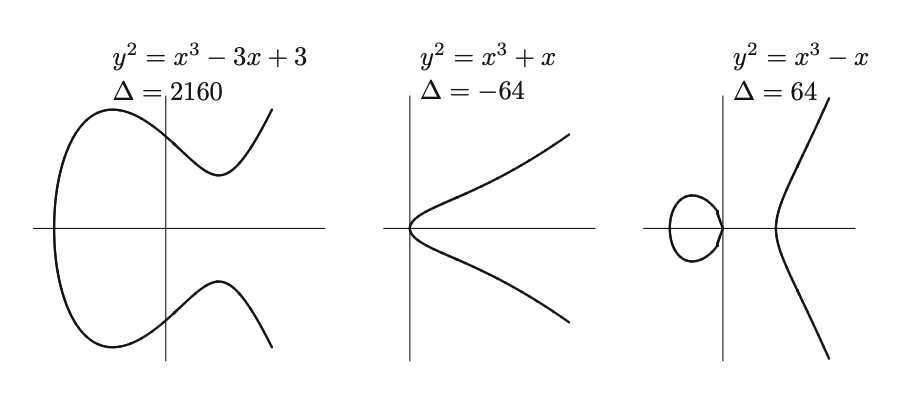
\includegraphics[scale=0.4]{Silverman_Fig31.png}\\
			\cite[Figure $3.1$]{Silverman-arithmetic-elliptic-curves}
		\end{column}\pause
		% Column 2    
		\begin{column}{.5\textwidth}
			\underline{Drinfeld Modules}\\
			
			Consider the rank $2$ lattice $\Lambda_z=\overline{\pi}(zA+A)\subset C.$\pause
			The associated \textbf{Drinfeld module of rank $2$} is given by \[\varphi^z(T)=TX+g(z)X^q+\Delta(z)X^{q^2},\]\pause
			the image of a ring homomorphism $\varphi^z: A\to C\{X^q\}$ where $C\{X^q\}$ is the non-commutative ring of $\bbF_q$-linear polynomials$/C.$ 
		\end{column}%
	\end{columns}
\end{frame}
	
\begin{frame}
	\frametitle{Moduli Problems}
	Let $\Gamma^1\leq \SL_2(\bbZ)$ and $\Gamma\leq \GL_2(A)$ be subgroups.\pause
	\[\left(\begin{array}{c}\text{quotient spaces}\\\Gamma^1\setminus\cH \text{ (resp. }\Gamma\setminus\Omega)\end{array}\right)
		\overset{\text{classify}}{\leftrightarrow}
		\left(\begin{array}{c}\text{families of elliptic curves}\\\text{(resp. Drinfeld modules of rank }2)\\\text{which have torsion info}\end{array}\right)
	\]
	\pause \\
	
	For example, \[\Gamma_0(N)\overset{def}{:=}\left\{\left(\begin{array}{cc}a&b\\c&d\end{array}\right): c\equiv 0\pmod{N}\right\}\]
	corresponds to the \textbf{moduli space} of \[\begin{cases}\text{elliptic curves}\\
	\text{Drinfeld modules of rank }2\end{cases}\quad\text{with an }N\text{-torsion subgroup.}\]
\end{frame}	
	
	
\begin{frame}
	\frametitle{Classical Modular Forms \& Curves}
	\begin{columns}
		\begin{column}{.3\textwidth}
			\centering
			\underline{Algebraic Modular Curve}\\
			$\sX_{\Gamma}$\\
			Deligne-Mumford (stacky) curve
		\end{column}\pause
		\begin{column}{.3\textwidth}
			\centering
			\underline{GAGA}\\
			$\leftrightarrow$
		\end{column}\pause
		\begin{column}{.3\textwidth}
			\centering
			\underline{Analytic Moduli Space}\\
			$\Gamma\setminus\cH^*$\\
			Compact Riemann surface (orbifold)
		\end{column}
	\end{columns}\pause
	
	\begin{definition}[{\cite[$1.1.2$]{Diamond-Shurman-first-course-modular-forms}}]
		A map $f:\cH\to \bbC$ is a \textbf{modular form of weight} $k\in \bbZ$ for $\Gamma\leq \SL_2(\bbZ)$ if \pause
		\begin{itemize}
			\item[$1.$] $f$ is holomorphic on $\cH$ and at cusps of $\Gamma$; and \pause
			\item[$2.$] $f(\gamma z)=(cz+d)^kf(z)$ for all $\gamma=\left(\begin{array}{cc}a&b\\c&d\end{array}\right)\in \Gamma$ and $z\in \cH.$
		\end{itemize}
	\end{definition}\pause
	We know (e.g.\ \cite[Chapter $6$]{VZB})
	\begin{align*}
	M(\Gamma)\overset{def}{:=}\bigoplus_{k\geq 0}M_k(\Gamma)&\overset{\sim}{\longrightarrow} \bigoplus_{k\geq 0} H^0(\sX_{\Gamma},\Omega^1_{\sX_{\Gamma}}(\Delta)^{\otimes k/2})\overset{def}{=:}R(\sX_{\Gamma},\Delta),\\\pause
	&f\mapsto fdz^{\otimes k/2}
	\end{align*}
\end{frame}	
	
\begin{frame}
	\frametitle{``Ingredients''}
	\begin{itemize}
		\item[$1.$] \textbf{(Log) Stacky Curve} $(\sX,\Delta)$ (\cite[Def $2.1$]{Landesman-Ruhm-Zhang-Spin-canonical-rings} and \cite[Ch $4$]{VZB}) 
		\begin{itemize}
			\item[-] a ``nice'' scheme $X$/$\overline{\bbK}$ of dimension $1,$ \pause together with ``fractional'' (\emph{stacky}) points $\frac{1}{e_1}P_1,\ldots, \frac{1}{e_r}P_r$ of $X$ with $e_i\in\bbZ_{\geq 2}$; \pause
			\item[-] a \emph{log divisor} is some $\Delta\in \operatorname{Div}(\sX)$ a sum of distinct points of $\sX$
		\end{itemize}
		\pause
		
		\item[$2.$] \textbf{(Ample) Line Bundle} 
		\begin{itemize}
			\item[-] e.g.\ $K_{\sX}\sim \Omega^1_{\sX}$ or $K_{\sX}+\Delta$ \pause 
			\item[-] gives an embedding of $\sX$ in projective space \pause
		\end{itemize} 
		
		\item[$3.$] \textbf{Modular forms ``$=$'' Sections} - \`a la ($f\mapsto fdz^{\otimes k/2}$) \pause
		
		\item[$4.$] \textbf{GAGA} - equivalences of categories: 
		\[\left(\begin{array}{c}\text{algebraic}\\
		\text{curves and bundles}\end{array}\right)\overset{\cong}{\to}\left(\begin{array}{c}\text{analytic}\\
		\text{curves and bundles}\end{array}\right)\]
	\end{itemize}
\end{frame}	

\begin{frame}
	\frametitle{Drinfeld Modular Forms \& Curves}
		\begin{columns}
		\begin{column}{.3\textwidth}
			\centering
			\underline{Algebraic Modular Curve}\\
			$\sX_{\Gamma}$\\
			Deligne-Mumford (stacky) curve
		\end{column}\pause
		\begin{column}{.3\textwidth}
			\centering
			\underline{rigid (stacky) GAGA}\\
			$\leftrightarrow$
		\end{column}\pause
		\begin{column}{.3\textwidth}
			\centering
			\underline{Analytic Moduli Space}\\
			$\Gamma\setminus(\Omega\cup\bbP^1(K))$\\
			compact rigid analytic stack
		\end{column}
	\end{columns}\pause
	
	\begin{definition}[{\cite[$(3.1)$]{Gekeler-Curves}}]
		Let $\Gamma\leq \GL_2(A)$ be a congruence subgroup. A \textbf{modular form} of \textbf{weight} $k\in \bbZ_{\geq0}$ and \textbf{type} $l\in \bbZ/((q-1) \bbZ)$ is a holomorphic function $f:\Omega\to C$ such that\pause 
		\begin{itemize}
			\item[$1.$] $f$ is holomorphic on $\Omega$ and at the cusps of $\Gamma$; and \pause
			\item[$2.$] $f(\gamma z)=\det(\gamma)^{-l}(cz+d)^kf(z)$ for all $\gamma=\left(\begin{array}{cc}a&b\\c&b\end{array}\right)\in \Gamma.$
		\end{itemize}
	\end{definition}
\end{frame}

\begin{frame}
	\frametitle{Geometry of Drinfeld Modular Forms $(1/3)$}
	\begin{columns} 
		% Column 1
		\begin{column}{.5\textwidth}
			Let $q$ be odd;\\
			Let $\Gamma\leq \GL_2(A)$;\\ 
			Let $\Gamma_2=\{\gamma\in \Gamma:\det(\gamma)\in (\bbF_q^{\times})^2\}.$ \pause\\
			Consider the cover of modular curves
			\begin{figure}[!h]\centering
				\begin{tikzcd}
						\sX_{\Gamma_2}\arrow[d]\\
						\sX_{\Gamma}
				\end{tikzcd}
			\end{figure}\pause
			When we compute the log canonical ring $R(\sX_{\Gamma_2}, 2\Delta)$ we get the following result.
		\end{column}\pause
		% Column 2    
		\begin{column}{.5\textwidth}
			\begin{theorem}[{\cite[$6.1$]{Franklin-geometry-Drinfeld-modular-forms}}]
				There is an isomorphism of graded rings \[M(\Gamma_2)\cong R(\sX_{\Gamma_2},\Omega^1_{\sX_{\Gamma_2}}(2\Delta)),\]\pause
				given by isomorphisms \[M_{k,l}(\Gamma_2)\to H^0(\sX_{\Gamma_2},\Omega^1_{\sX_{\Gamma_2}}(2\Delta)^{\otimes k/2})\] of form $f\mapsto f(dz)^{\otimes k/2},$ \pause where \\$k\equiv 2l\pmod{q-1}.$ 
			\end{theorem}
		\end{column}
	\end{columns}
\end{frame}

\begin{frame}
	\frametitle{Geometry of Drinfeld Modular Forms $(2/3)$}
	\begin{columns} 
		% Column 1
		\begin{column}{.5\textwidth}
			Let $q$ be odd;\\
			Let $\Gamma\leq \GL_2(A)$;\\ 
			Let $\Gamma_2=\{\gamma\in \Gamma:\det(\gamma)\in (\bbF_q^{\times})^2\}.$\\
			Consider the cover of modular curves\\
			\begin{figure}[!h]\centering
				\begin{tikzcd}
					\sX_{\Gamma_2}\arrow[d]\\
					\sX_{\Gamma}
				\end{tikzcd}
			\end{figure}\pause
			When we compare the modular forms for $\Gamma$ and $\Gamma_2$ we find the following.
		\end{column}\pause
		% Column 2    
		\begin{column}{.5\textwidth}
			\begin{theorem}[{\cite[$6.2$]{Franklin-geometry-Drinfeld-modular-forms}}]
				We have $M(\Gamma)\cong M(\Gamma_2),$ \pause
				with \[M_{k,l}(\Gamma_2)=M_{k,l_1}(\Gamma)\oplus M_{k,l_2}(\Gamma)\] on each component,\pause where $l_1,l_2$ are the solutions to $k\equiv 2l\pmod{q-1}.$ 
			\end{theorem}
		\end{column}
	\end{columns}
\end{frame}	

\begin{frame}
	\frametitle{Geometry of Drinfeld Modular Forms $(3/3)$}
	\begin{columns} 
		% Column 1
		\begin{column}{.5\textwidth}
			Let $q$ be odd;\\
			$\Gamma\leq \GL_2(A)$;\\ 
			$\Gamma_1=\{\gamma\in \Gamma:\det(\gamma)=1\}.$\\
			Suppose that $\Gamma_1\leq \Gamma'\leq \Gamma.$ \pause \\
			Consider the cover of modular curves
			\begin{figure}[!h]\centering
				\begin{tikzcd}
					\sX_{\Gamma'}\arrow[d]\\
					\sX_{\Gamma}
				\end{tikzcd}
			\end{figure}\pause
			When we compare the modular forms for $\Gamma$ and $\Gamma'$ we find the following generalization of \cite[Theorem $6.2$]{Franklin-geometry-Drinfeld-modular-forms}.
		\end{column}\pause
		% Column 2    
		\begin{column}{.5\textwidth}
			\begin{theorem}[{\cite[$6.12$]{Franklin-geometry-Drinfeld-modular-forms}}]
				We have $M(\Gamma)\cong M(\Gamma'),$ \pause
				and each component $M_{k,l}(\Gamma')$ is some direct sum of components $M_{k,l'}(\Gamma)$ for some nontrivial $l'.$
			\end{theorem}
		\end{column}
	\end{columns}	
\end{frame}

\begin{frame}
	\frametitle{Conclusion}
	\centering
	Thank you!\\
	
	Further details available at \href{https://arxiv.org/abs/2310.19623}{arXiv:$2310.19623$} 
\end{frame}

\begin{frame}[allowframebreaks]
	\frametitle{References}
	\bibliography{bibliography}
	\bibliographystyle{amsalpha}
\end{frame}

	
\end{document}